\chapter{Parametric Exploration of the \emph{EvoTSC} Model}
\label{chap:param}

In this chapter, I present several sets of additional evolutionary simulations.
In these simulations, I explore the robustness of the characteristics of evolving populations to variations in the \emph{EvoTSC} model, measuring whether populations are able to evolve differentiated gene expression patterns as a response to different environments, and comparing their speed of evolution with that of the main runs presented in Chapter~\ref{chap:ploscb}.
I first explore changing different parameters, presented in Table~\ref{tab:param:params}: the maximum interaction distance for the transcription-supercoiling coupling, the mean intergenic distance, the strength of the environment-caused shift in background supercoiling, and the number of genes on the genome.
I then discuss the effect of introducing indels in intergenic sections as a new mutational operator in the model.

\begin{table}
\begin{center}
\begin{tabular}{l c r r}
\toprule
\textbf{Parameter} & \textbf{Symbol} & \textbf{Value} & \textbf{Replicates} \\
\midrule
Interaction distance \textbf{OK} & $d_{max}$ & \textbf{5 kb} & \textbf{30}\\
& & 25 kb & 15\\
\midrule
& & 10 bp& 15\\
Mean intergenic distance \textbf{OK} & $d_{mean}$ & \textbf{125 bp} & \textbf{30} \\
& & 1,000 bp & 15\\
& & 10,000 bp & 15 \\
\midrule
& & 0.0001 & 15\\
Environment supercoiling \textbf{PAS OK}& $\delta\sigma_{A/B}$ & 0.001 & 15\\
& & \textbf{0.01} & \textbf{30}\\
\midrule
Number of genes \textbf{PAS OK} & $n$ & \textbf{60} & \textbf{30} \\
& & 30 & 15 \\
\bottomrule
\end{tabular}
\end{center}
\caption[Table of parameter values explored in additional \emph{EvoTSC} simulations]{Table of the parameters and associated values explored in additional experiments (separated by horizontal lines).
For each experiment, the row in bold font corresponds to the parameter values used in the main run described in Chapter~\ref{chap:ploscb}, and is shown for reference.}
\label{tab:param:params}
\end{table}

\section{Interaction Distance}

The size of the topological domains of bacterial genomes, inside which DNA supercoils can freely propagate, has historically been estimated to be on the order of a few thousand base pairs~\citep{elhanafi2000,kouzine2013}.
Recent work has however suggested that topological domains could be up to ten times larger than this, reaching up to 25 kb~\citep{visser2022}.
As this distance sets a limit to the number of genes that can interact through the transcription-supercoiling coupling, it plays an important role in the structure of the supercoiling-mediated gene regulatory networks.

A larger supercoiling interaction distance increases the number of neighboring genes that impact a given gene.
It could therefore make genomic inversions more deleterious by making them disrupt a larger part of the regulatory networks at their boundaries, but could also allow more robust regulatory networks to evolve through a higher connectivity.

\begin{figure}[H]
\centering
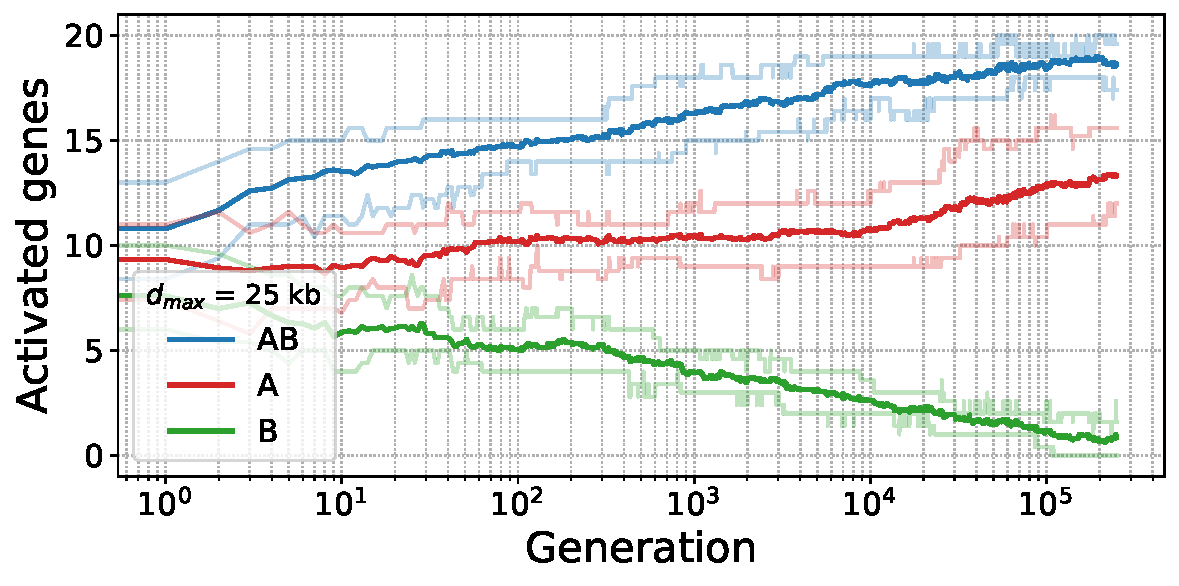
\includegraphics[width=0.495\textwidth]{param/interaction-25k/gene_activity_env_A.pdf}
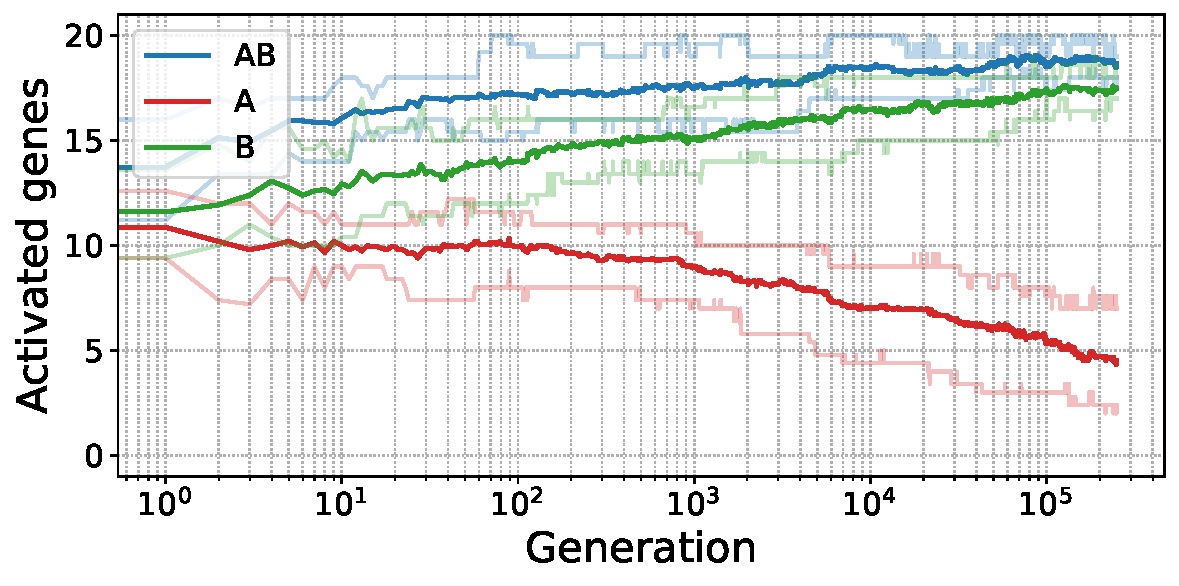
\includegraphics[width=0.495\textwidth]{param/interaction-25k/gene_activity_env_B.pdf}
\caption[Evolution of the number of active genes in each environment with an interaction distance of 25 kb]{Evolution of the number of active genes in environment A (left) and environment B (right), with an interaction distance of 25 kb.}
\label{fig:param:inter25k-activity-by-env}
\end{figure}

Figure~\ref{fig:param:inter25k-activity-by-env} shows the evolution of the number of active genes of each type in the simulations with the interaction distance of 25 kb, over 250,000 generations.
As in the main run, the number of active genes of each type evolves towards their respective target.
Differentiated activation patterns can therefore still evolve even when the topological domains are 5 times larger.

\begin{figure}[H]
\centering
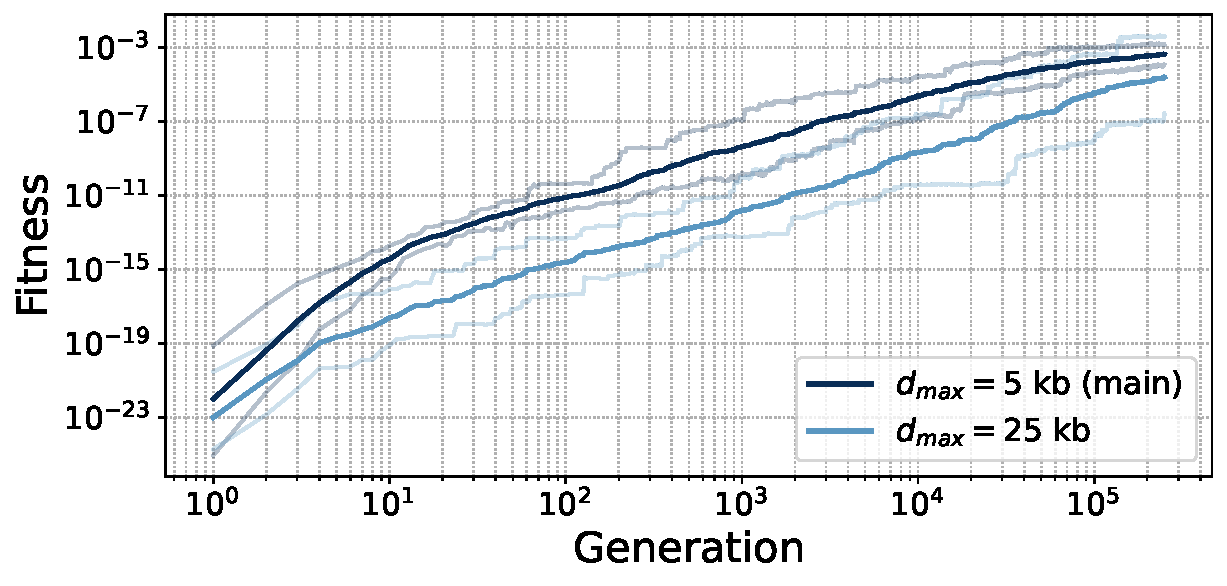
\includegraphics[width=0.75\textwidth]{param/interaction-25k/fitness_all_with_main.pdf}
\caption[Average fitness during evolution with an interaction distance of 25 kb]{Average fitness during evolution with an interaction distance of 25 kb (yellow).
The main run is presented in purple for comparison.}
\label{fig:param:inter25k-fitness}
\end{figure}

Figure~\ref{fig:param:inter25k-fitness} shows the evolution of the average fitness of the best individual in each replicate of the simulation with a larger interaction distance, compared with the evolution of fitness in the main run, over 250,000 generations.
While fitness is systematically lower throughout evolution with the larger interaction distance, it nonetheless follows a qualitatively similar pattern, and fitness keeps increasing until the end of the runs, suggesting that it could eventually reach the same value as in the main run (presented in full in Figure~\ref{fig:ploscb:main_fitness}).

\begin{figure}[H]
\centering
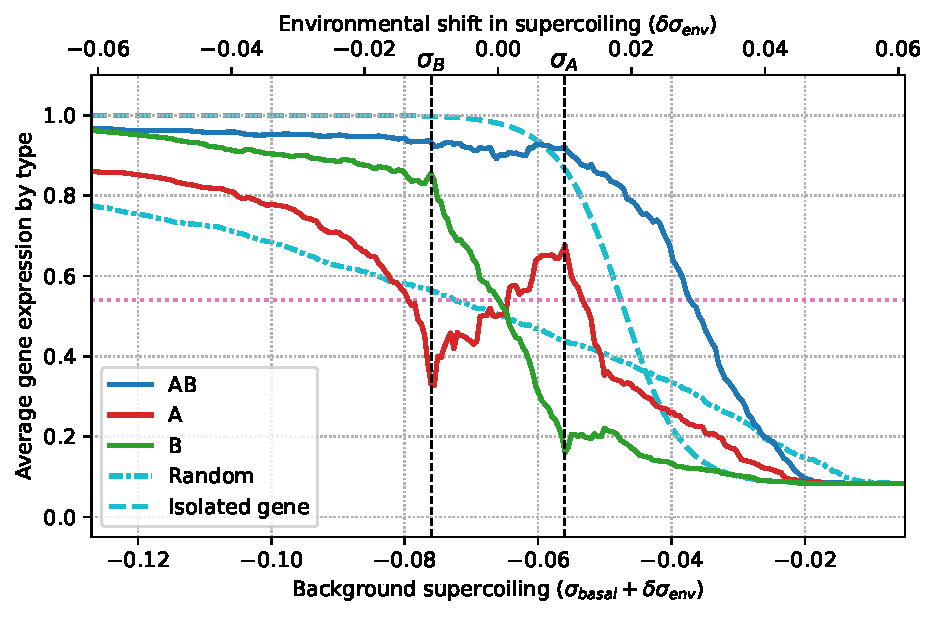
\includegraphics[width=0.9\textwidth]{param/interaction-25k/activity_sigmas_avg.pdf}
\caption[Average gene expression as a function of background supercoiling with an interaction distance of 25 kb]{Average gene expression by type as a function of background supercoiling, with an interaction distance of 25 kb.
The dash-dotted line represents the average expression of genes on a random genome with an interaction distance of 25 kb.}
\label{fig:param:inter25k-activ-by-sigma}
\end{figure}

Figure~\ref{fig:param:inter25k-activ-by-sigma} shows the average gene expression by type of evolved individuals, as a function of the background supercoiling level.
As in the main run, \emph{A} genes display a relaxation-activated phenotype.
\emph{AB} and \emph{B} genes are relaxation-inhibited, but nonetheless display quite different behaviors than the (dash-dotted light blue) curve for genes on a random genome with the same parameters, which present a much flatter response curve to background supercoiling than with the default interaction distance of 5 kb (shown in Figure~\ref{fig:ploscb:activity_by_sigma}).

\begin{figure}[H]
  \begin{subfigure}[t]{0.495\textwidth}
    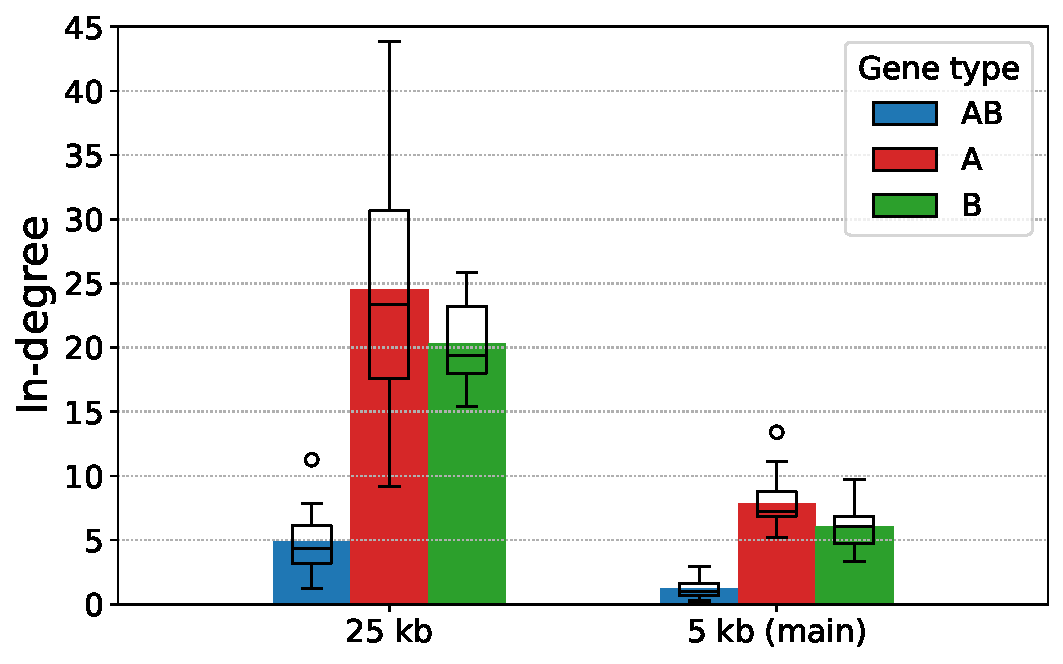
\includegraphics[width=\textwidth]{param/interaction-25k/effective_graph_combined_in_degree.pdf}
  \end{subfigure}
  \begin{subfigure}[t]{0.495\textwidth}
    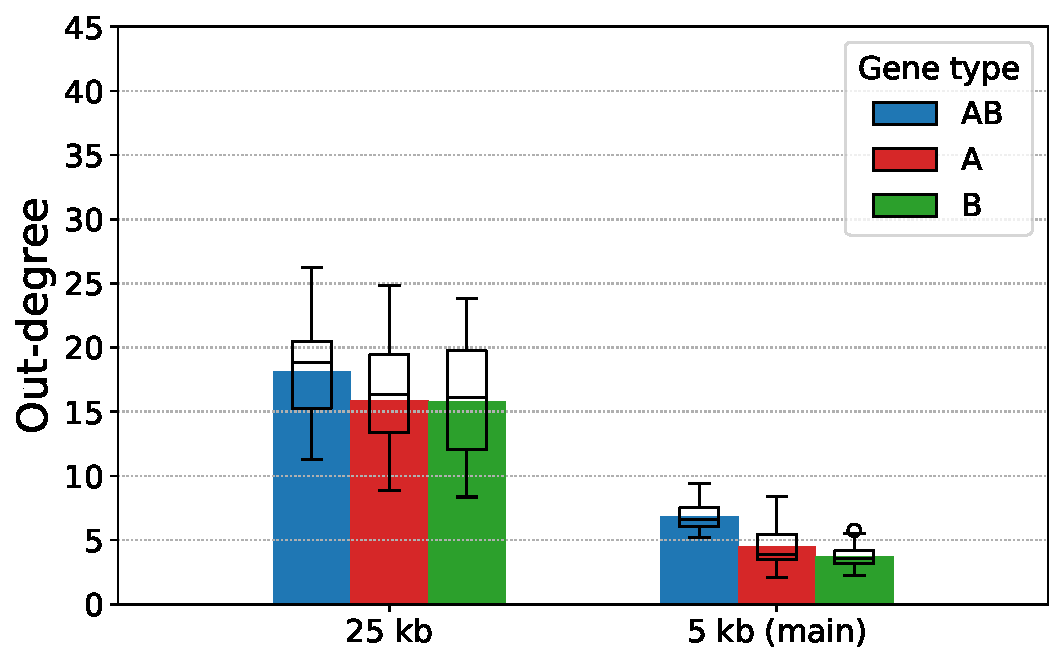
\includegraphics[width=\textwidth]{param/interaction-25k/effective_graph_combined_out_degree.pdf}
  \end{subfigure}
  \caption[Average in- and out-degree of effective interaction graph nodes with an interaction distance of 25 kb]{Average out-degree (left) and in-degree (right) of the genes in the effective interaction graph, separated by gene type, for individuals with an interaction distance of 5 kb (main run) or 25 kb.}
  \label{fig:param:inter25k-degree}
\end{figure}

Figure~\ref{fig:param:inter25k-degree} finally presents the average in- and out-degree of the genes in the effective interaction graph obtained with gene knockouts, compared to the same data from the main run.
As could be expected, the gene regulatory networks are much more connected with the larger interaction distance, but the behavior per gene type remains qualitatively the same as in the main run.


\section{Mean Intergenic Size}

Then, I present simulations with varying mean intergenic distances, in order to test the robustness of the results with regard to different bacterial gene densities~\citep{kuo2009}.


\begin{figure}
\centering
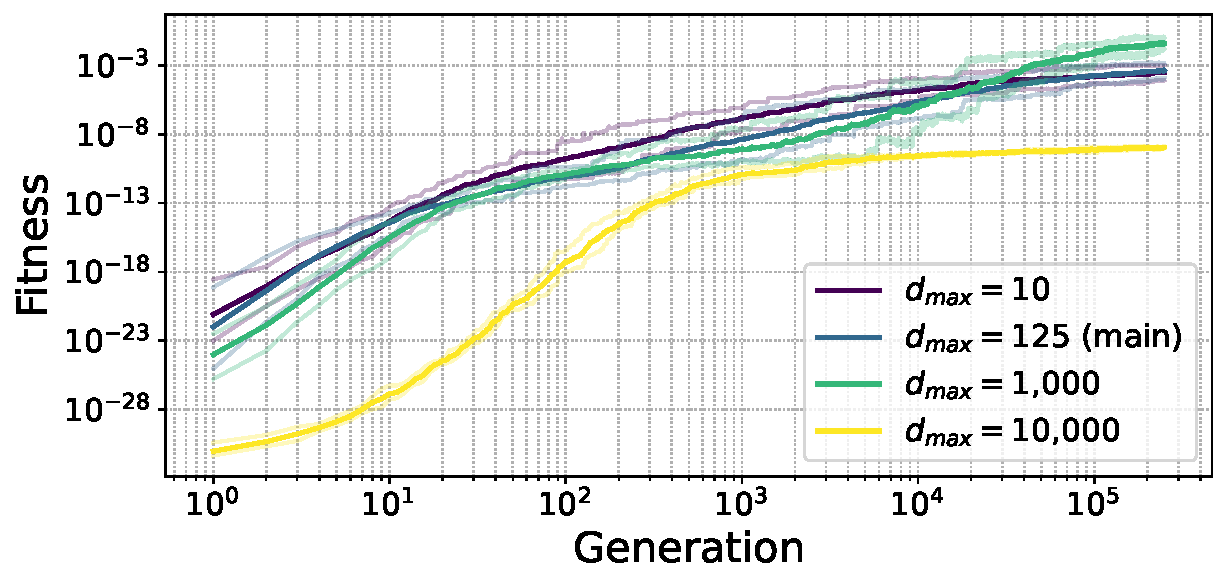
\includegraphics[width=0.75\textwidth]{param/mean-intergene/fitness_all_with_main.pdf}
\caption{Evolution of the fitness during evolution for average intergenic sizes of 10 bp \textbf{REFAIRE AVEC 15 REP}, 125 bp (main run), 1,000 bp, and 10,000 bp.}
%\label{}
\end{figure}

\begin{figure}
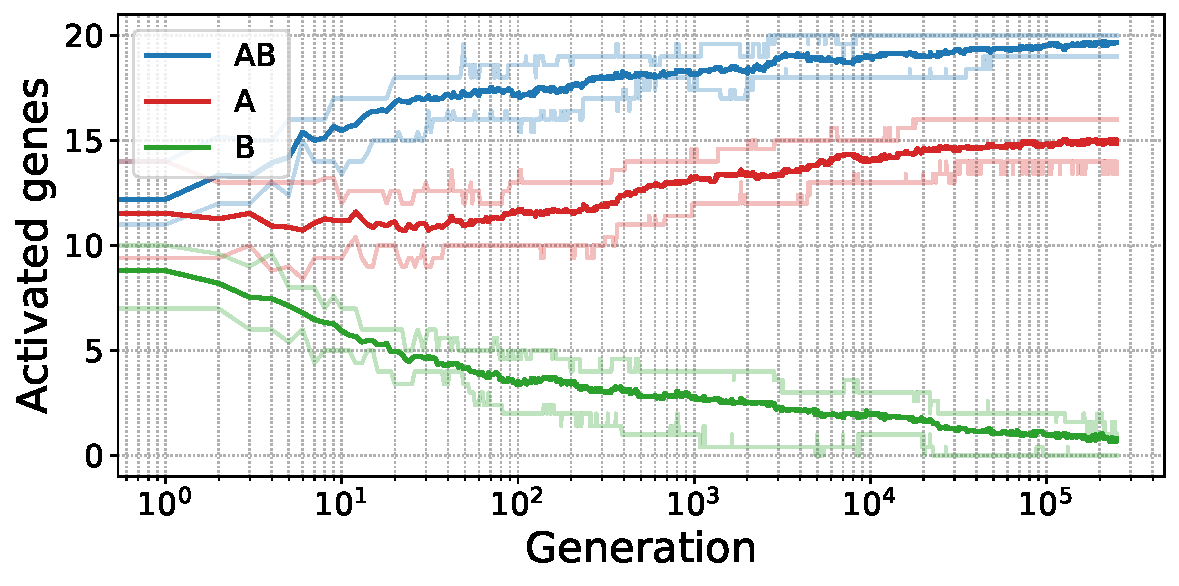
\includegraphics[width=0.495\textwidth]{param/mean-intergene/inter-0.01k/gene_activity_env_A.pdf}
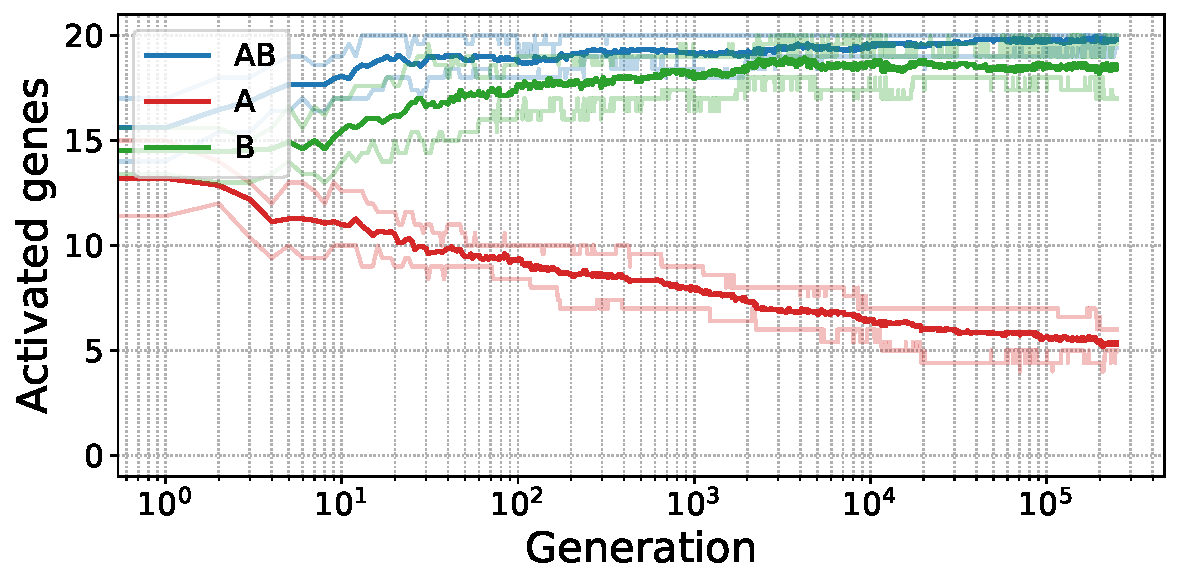
\includegraphics[width=0.495\textwidth]{param/mean-intergene/inter-0.01k/gene_activity_env_B.pdf}

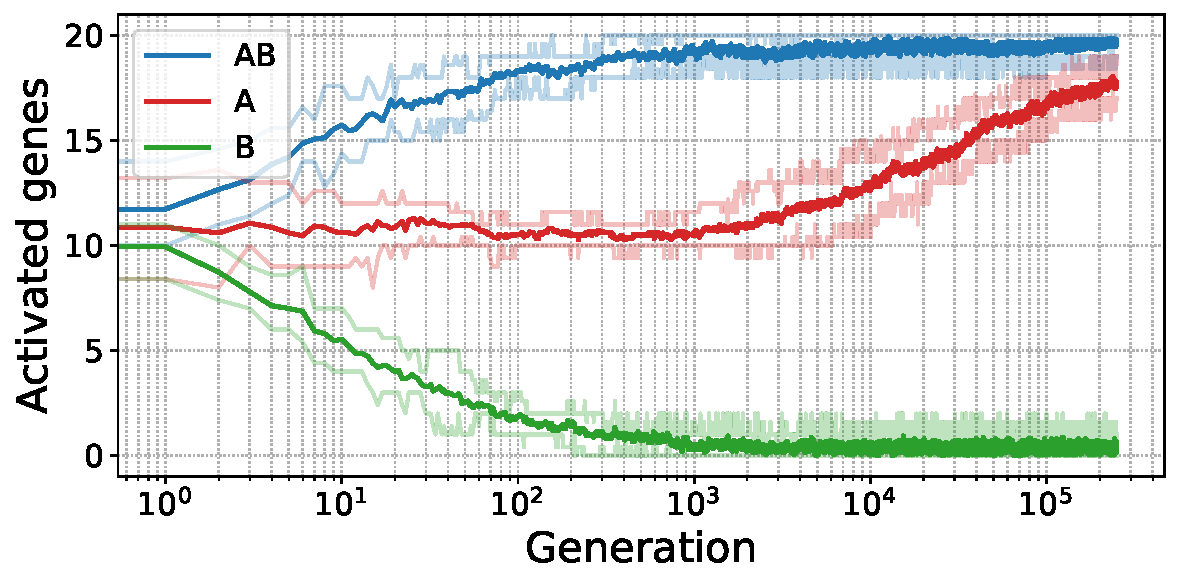
\includegraphics[width=0.495\textwidth]{param/mean-intergene/inter-1k/gene_activity_env_A.pdf}
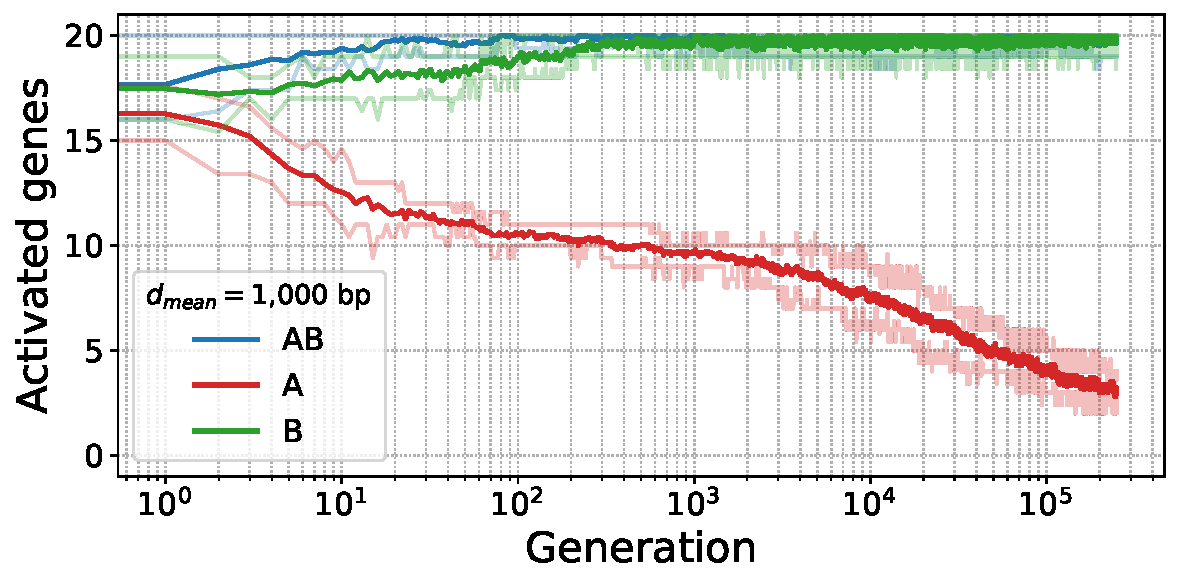
\includegraphics[width=0.495\textwidth]{param/mean-intergene/inter-1k/gene_activity_env_B.pdf}

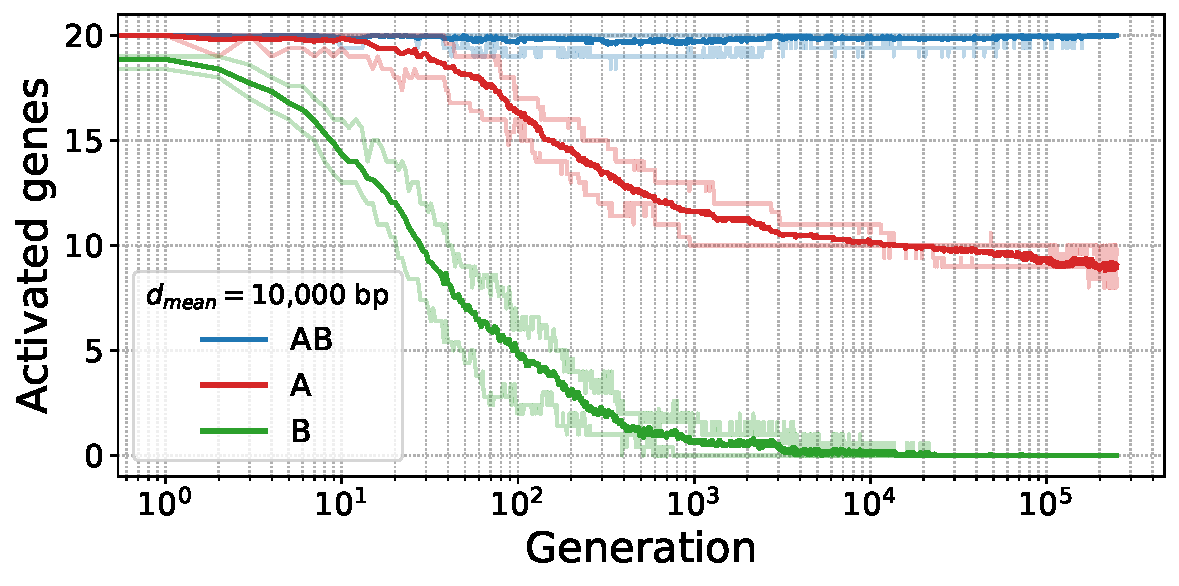
\includegraphics[width=0.495\textwidth]{param/mean-intergene/inter-10k/gene_activity_env_A.pdf}
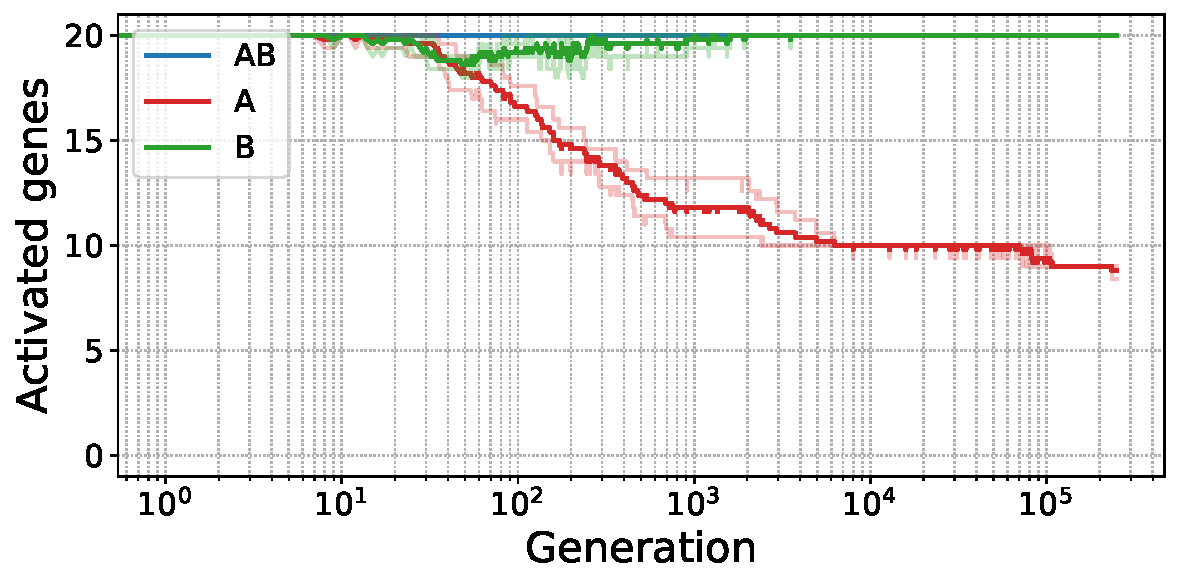
\includegraphics[width=0.495\textwidth]{param/mean-intergene/inter-10k/gene_activity_env_B.pdf}
\caption{Evolution of the number of activated genes in environment A (left) and B (right) during evolution, for average intergenic sizes of 10 bp (top) \textbf{REFAIRE AVEC 15 REP}, 1,000 bp (middle), and 10,000 bp (bottom) base pairs.}
%\label{}
\end{figure}

\begin{figure}

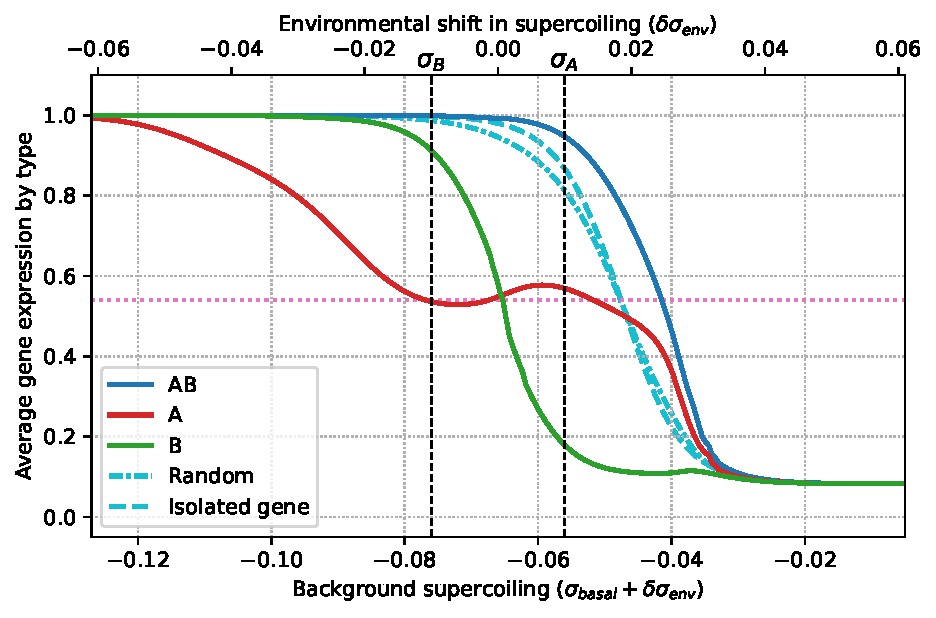
\includegraphics[width=0.9\textwidth]{param/mean-intergene/inter-10k/activity_sigmas_avg.pdf}
\caption{Average gene expression as a function of background supercoiling, with an intergenic distance of 10 kb.}
\end{figure}


\begin{figure}

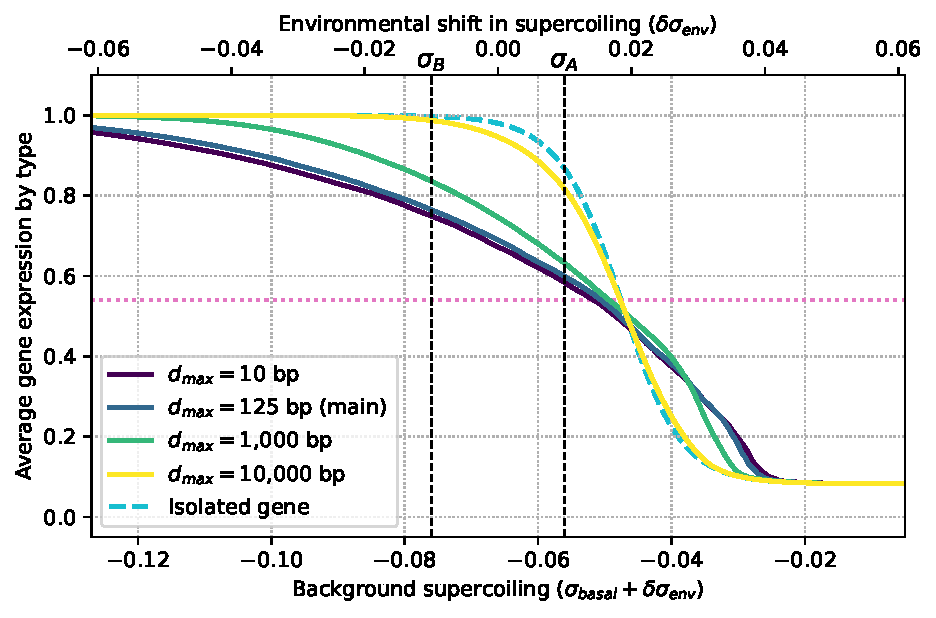
\includegraphics[width=\textwidth]{param/mean-intergene/random_activ_per_sigma.pdf}
\caption{expression level of random genes.}
\end{figure}








\FloatBlock

\section{Environmental Shift in Supercoiling}


As in section~\ref{sec:alife:param_explor}, I then present evolutionary simulations with smaller environmental shifts in supercoiling, in order to test the sensitivity of the gene regulatory networks that emerge.


\begin{figure}
\centering
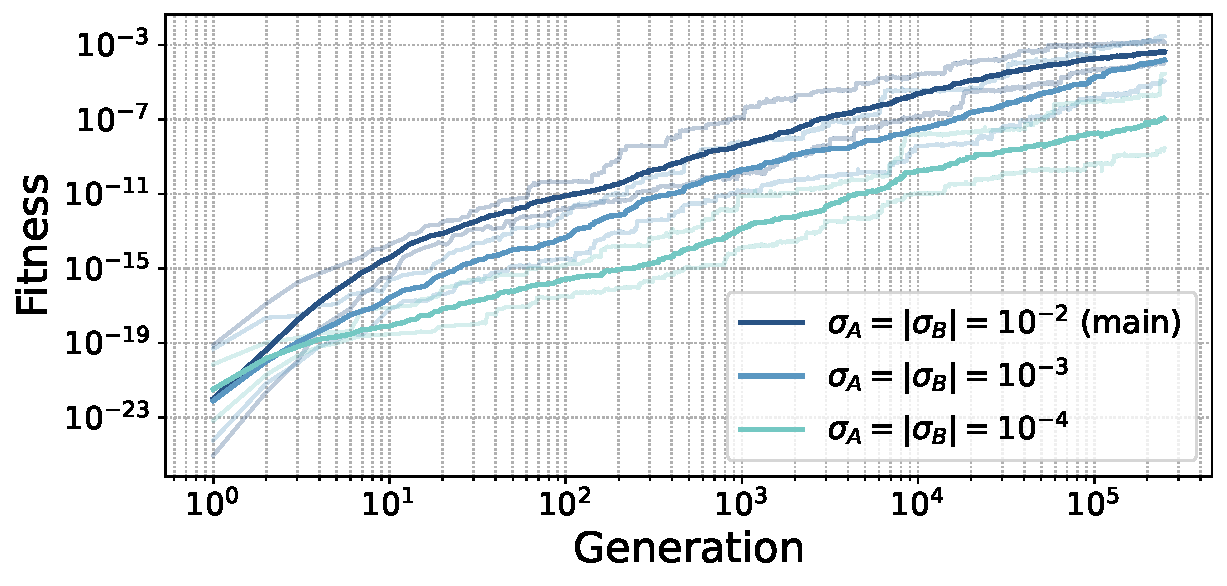
\includegraphics[width=0.75\textwidth]{param/sigma/fitness_all_with_main.pdf}
\caption{Evolution of the fitness during evolution for with environmental supercoiling shifts $\sigma_A = 0.001$ and $\sigma_B = -0.001$ (top) and $\sigma_A = 0.001$ and $\sigma_B = -0.001$ (bottom) \textbf{REFAIRE AVEC 15 REP}.}
%\label{}
\end{figure}


\begin{figure}
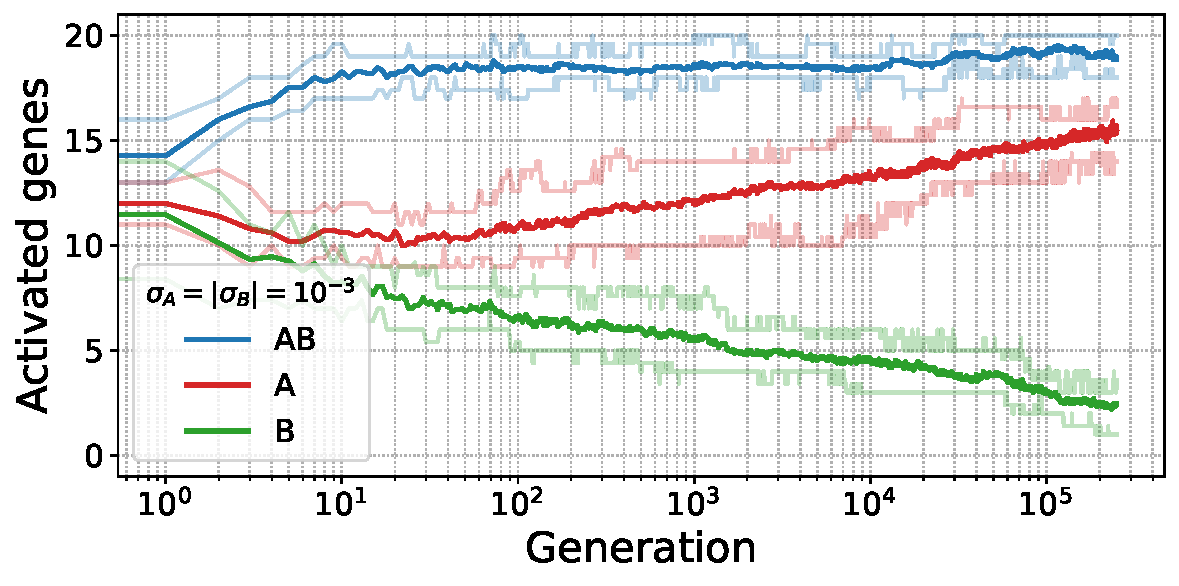
\includegraphics[width=0.495\textwidth]{param/sigma/sigma-1e-3/gene_activity_env_A.pdf}
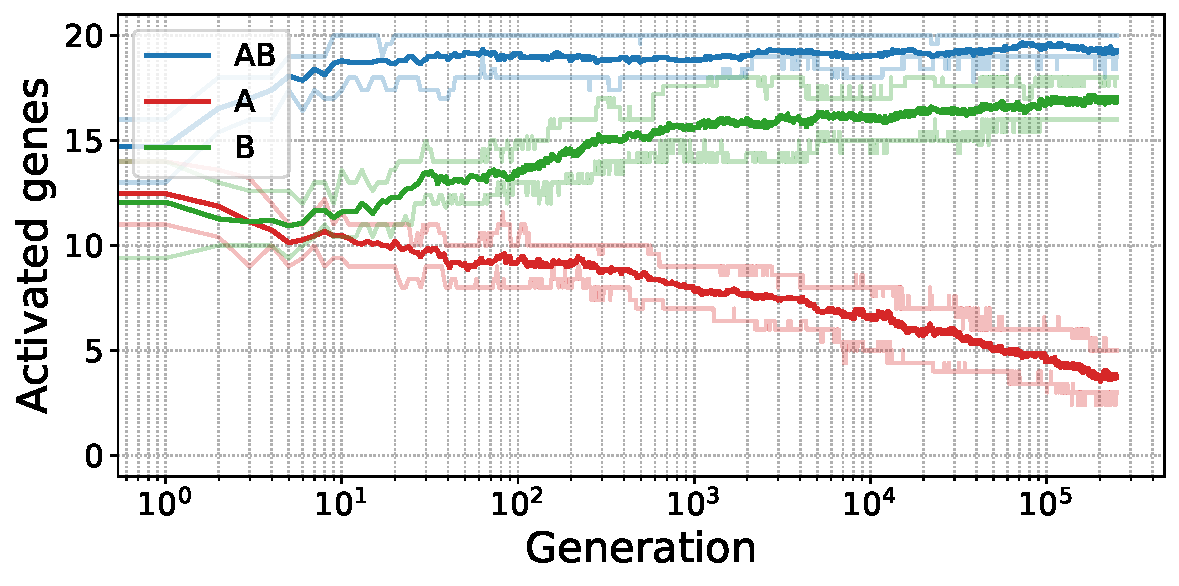
\includegraphics[width=0.495\textwidth]{param/sigma/sigma-1e-3/gene_activity_env_B.pdf}

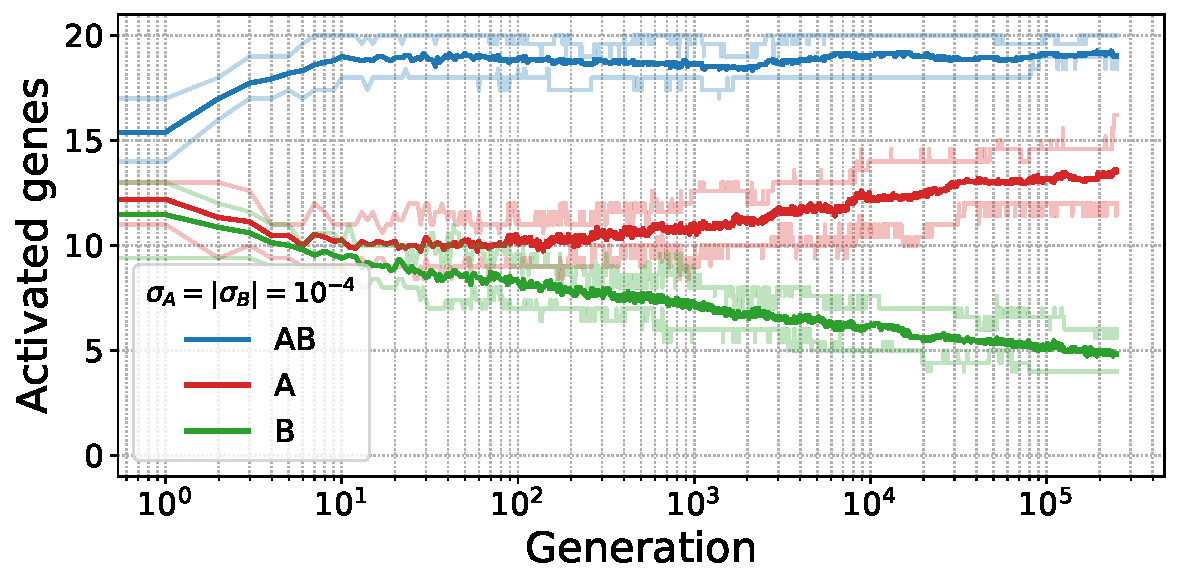
\includegraphics[width=0.495\textwidth]{param/sigma/sigma-1e-4/gene_activity_env_A.pdf}
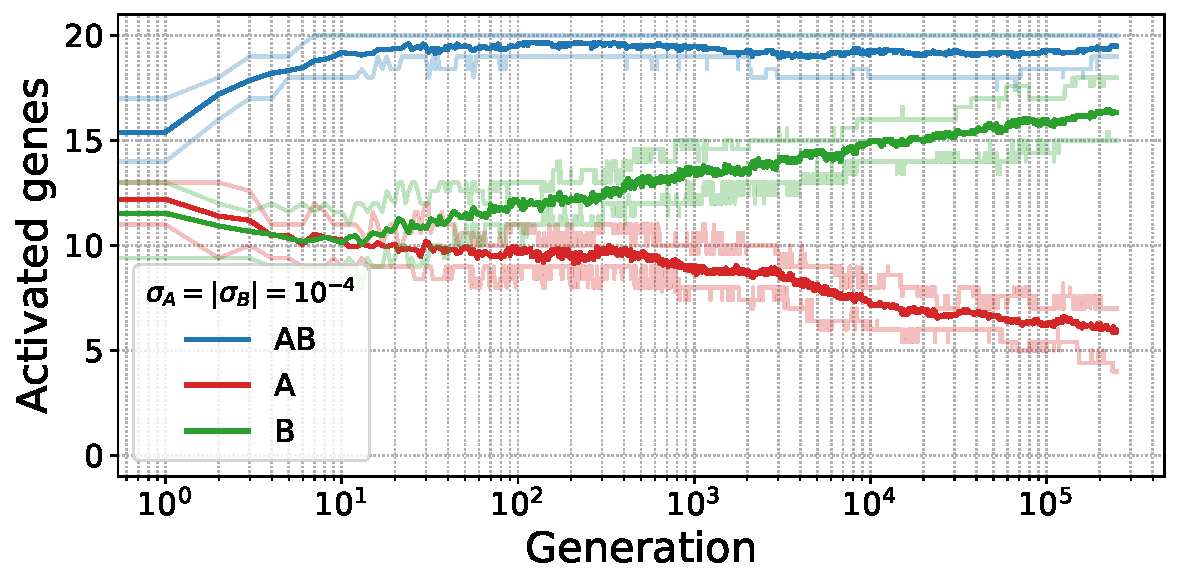
\includegraphics[width=0.495\textwidth]{param/sigma/sigma-1e-4/gene_activity_env_B.pdf}
\caption[Evolution of the number of active genes in each environment with an absolute environmental supercoiling shift of 0.001 or 0.0001]{Evolution of the number of active genes in environment A (left) and environment B (right), with environmental supercoiling shifts $\sigma_A = 0.001$ and $\sigma_B = -0.001$ (top) and $\sigma_A = 0.001$ and $\sigma_B = -0.001$ (bottom). \textbf{RELANCER AVEC 15 REP}}
\label{}
\end{figure}

Evolution still works with a 10 times or 100 times smaller shift in supercoiling caused by the environment.

\begin{figure}
\centering
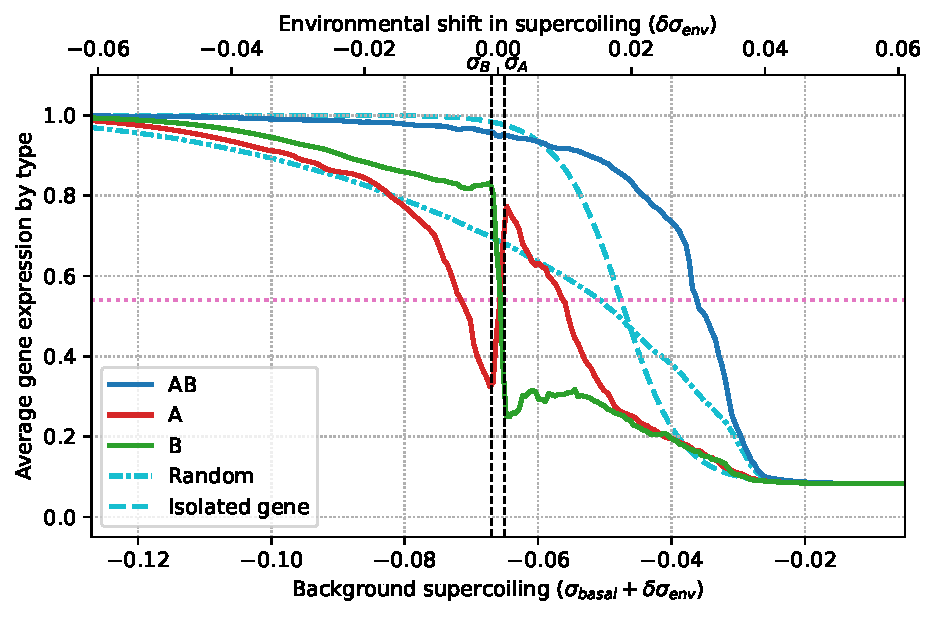
\includegraphics[width=0.9\textwidth]{param/sigma/sigma-1e-3/activity_sigmas_avg.pdf}
\caption[Average gene expression as a function of background supercoiling, with an absolute environmental supercoiling shift of 0.001]{Average gene expression as a function of background supercoiling, with environmental supercoiling shifts $\sigma_A = 0.001$ and $\sigma_B = -0.001$.\textbf{RELANCER AVEC 15 REP}}
\end{figure}

\begin{figure}
\centering
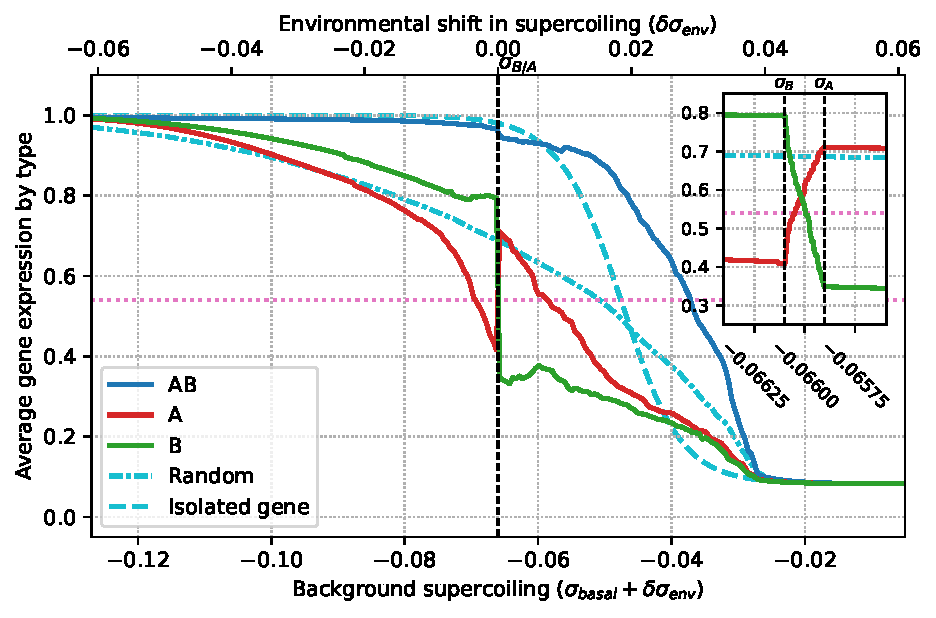
\includegraphics[width=0.9\textwidth]{param/sigma/sigma-1e-4/activity_sigmas_avg.pdf}
\caption[Average gene expression as a function of background supercoiling, with an absolute environmental supercoiling shift of 0.0001]{Average gene expression as a function of background supercoiling, with environmental supercoiling shifts $\sigma_A = 0.0001$ and $\sigma_B = -0.0001$.\textbf{RELANCER AVEC 15 REP}}
\end{figure}

In all these cases, everything still works.






\FloatBlock

\section{Number of Genes}

Finally, I present runs with a larger number of genes


\begin{figure}[H]
\centering
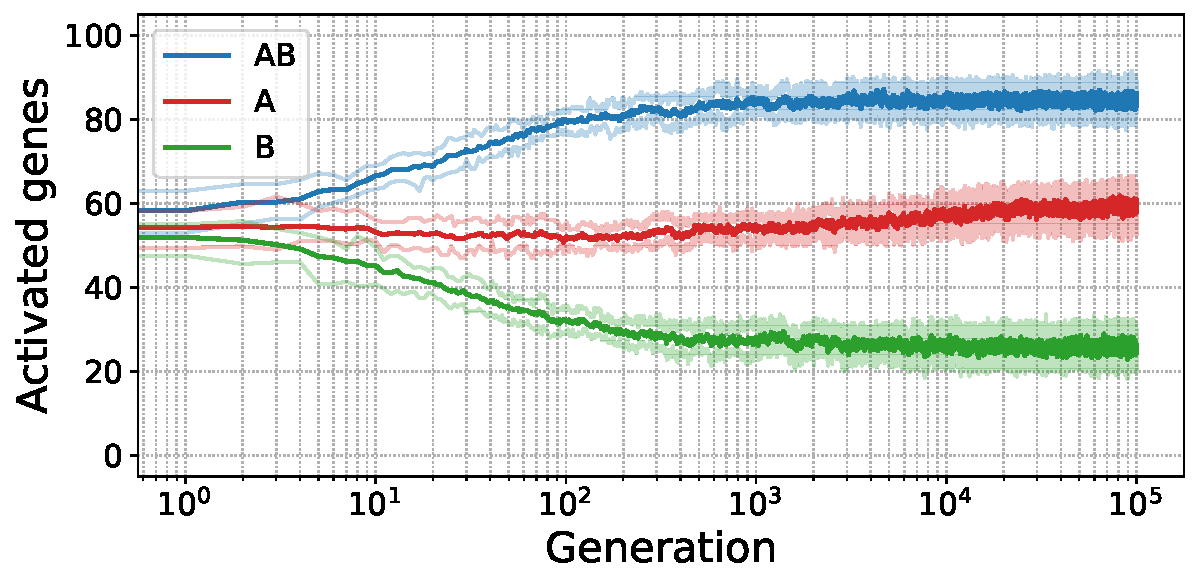
\includegraphics[width=0.495\textwidth]{param/300-genes/gene_activity_env_A.pdf}
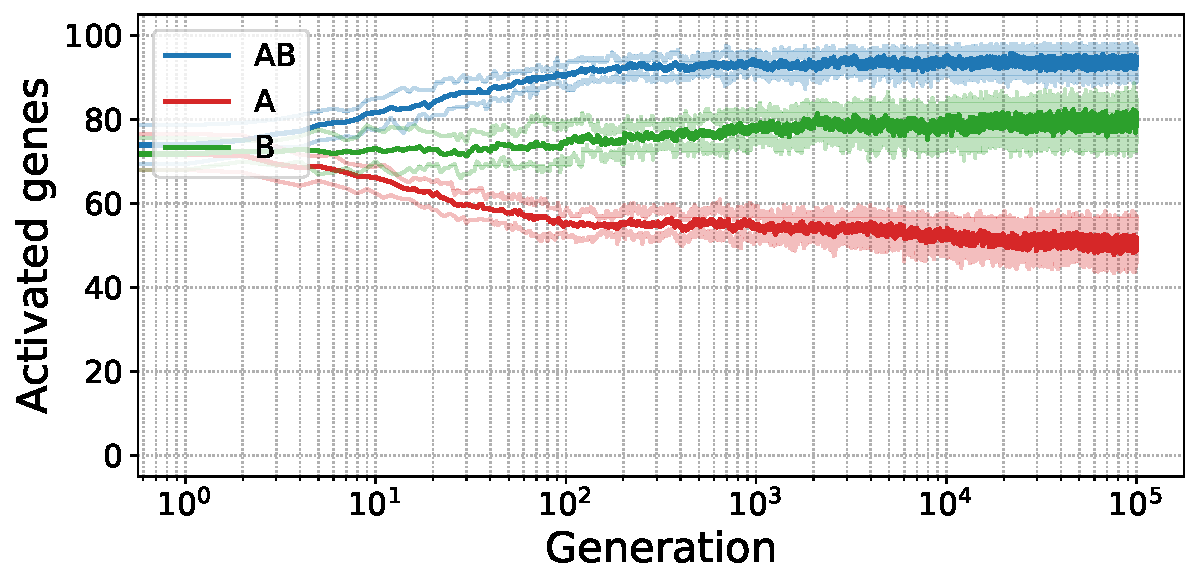
\includegraphics[width=0.495\textwidth]{param/300-genes/gene_activity_env_B.pdf}
\caption[Evolution of the number of active genes in each environment, with a 300-gene genome]{Evolution of the number of active genes in environment A (top) and environment B (bottom), with an interaction distance of 25 kb.}
%\label{fig:param:inter25k-active}
\end{figure}

\begin{figure}[H]
\centering
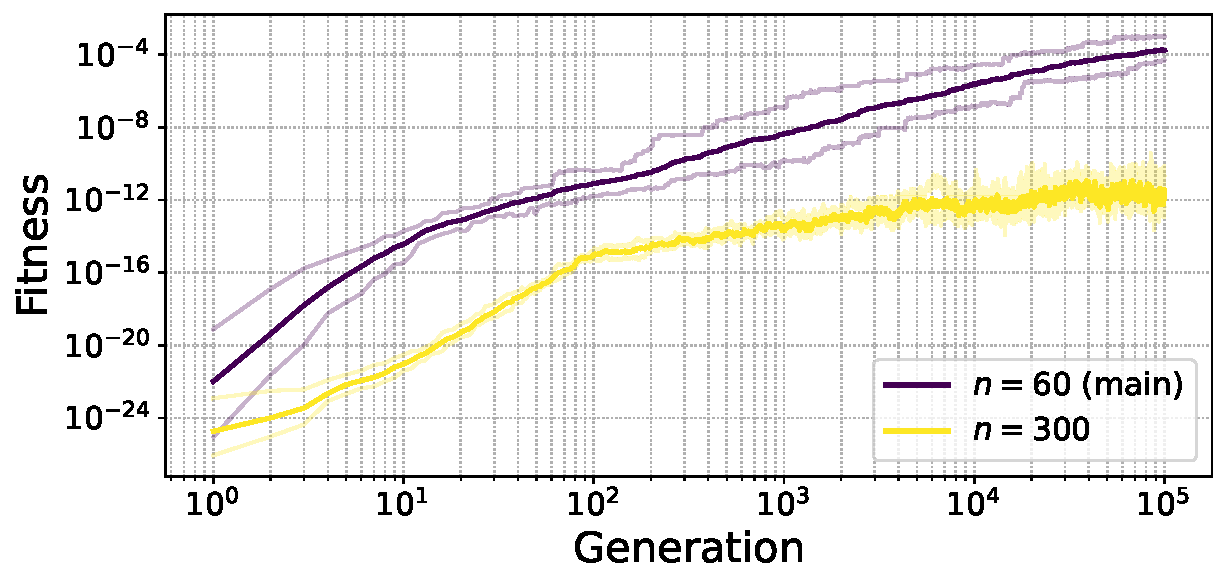
\includegraphics[width=0.75\textwidth]{param/300-genes/fitness_all_with_main.pdf}
\caption[Average fitness during evolution, with a 300-gene genome]{Average fitness during evolution, with a 300-gene genome.}
\end{figure}


\begin{figure}[H]
\centering
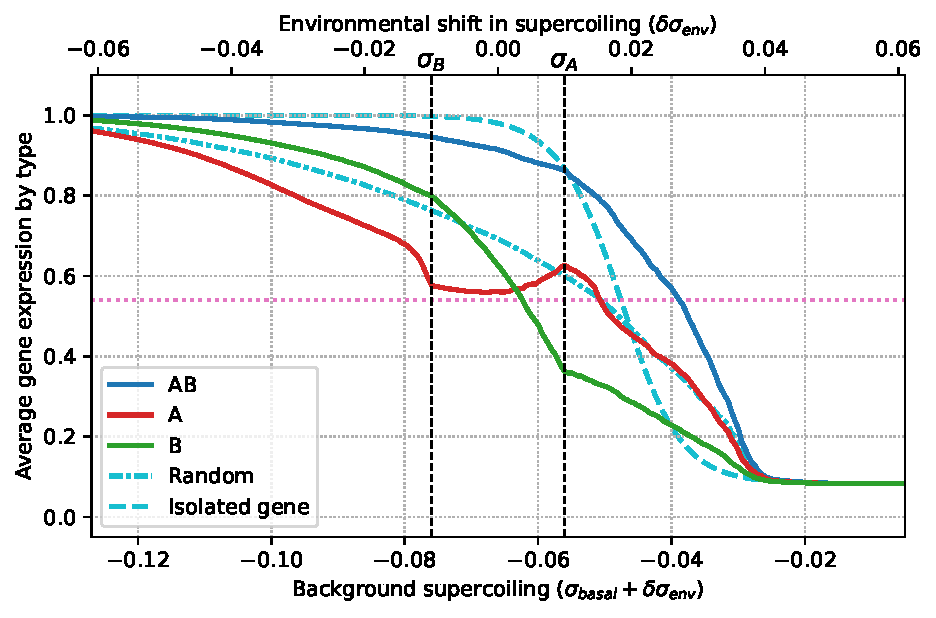
\includegraphics[width=0.9\textwidth]{param/300-genes/activity_sigmas_avg.pdf}
\caption[Average gene expression as a function of background supercoiling, with a 300-gene genome]{Average gene expression as a function of background supercoiling, with a 300-gene genome.}
%\label{fig:param:inter25k-activ-by-sigma}
\end{figure}








\FloatBlock

\section{Mutation in Intergenic Size}


\begin{figure}[H]
  \centering
  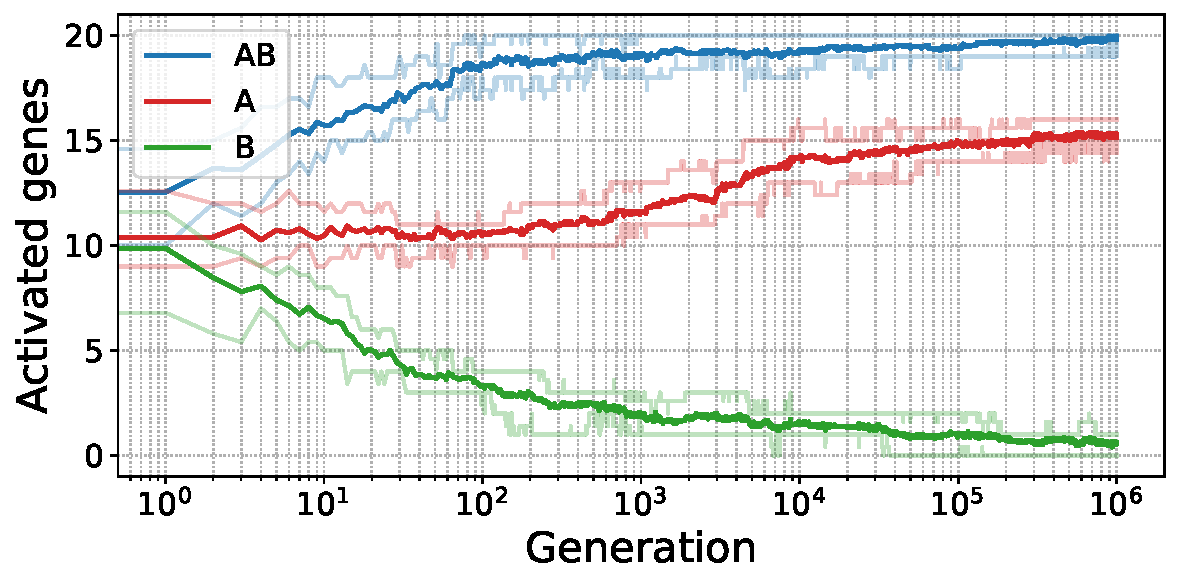
\includegraphics[width=0.495\textwidth]{param/evolve-intergene/gene_activity_env_A.pdf}
  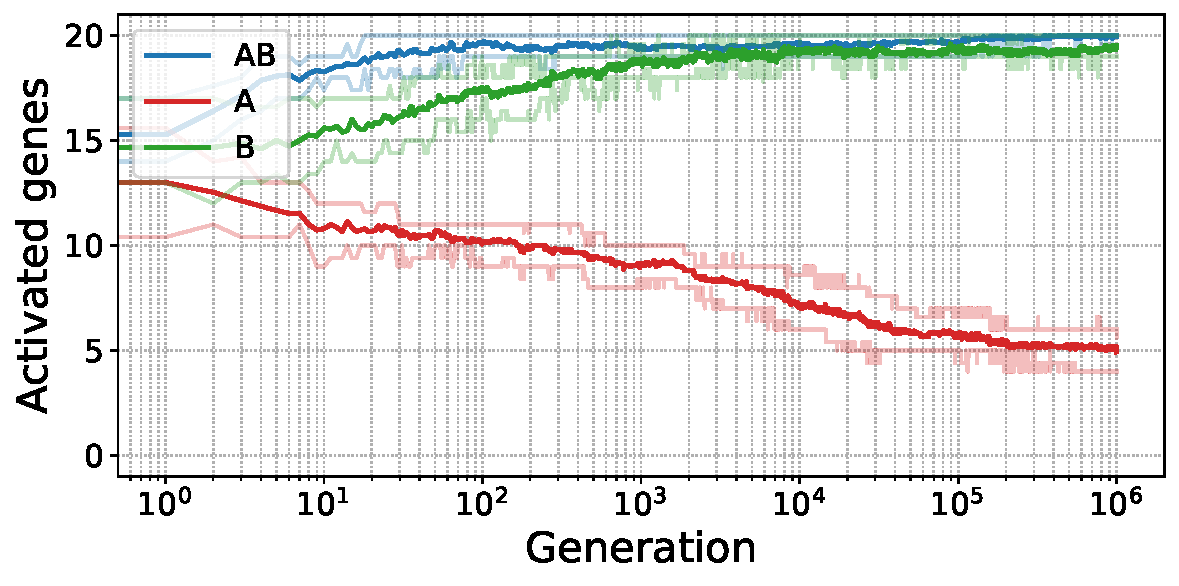
\includegraphics[width=0.495\textwidth]{param/evolve-intergene/gene_activity_env_B.pdf}
  \caption[Evolution of the number of active genes in each environment, with intergenic distance mutations]{Evolution of the number of active genes in environment A (top) and environment B (bottom), with intergenic distance mutations.}
  %\label{fig:param:inter25k-active}
  \end{figure}


\begin{figure}
\begin{elasticrow}[width=\textwidth]
\elasticfigure{param/evolve-intergene/fitness_all_with_main.pdf}
\elasticfigure{param/evolve-intergene/intergenic_size_all.pdf}
\end{elasticrow}
\caption[Average fitness and intergenic size during evolution, with intergenic distance mutations]{Fitness and average genome size during evolution, with intergenic distance mutations.}
\end{figure}



\begin{figure}
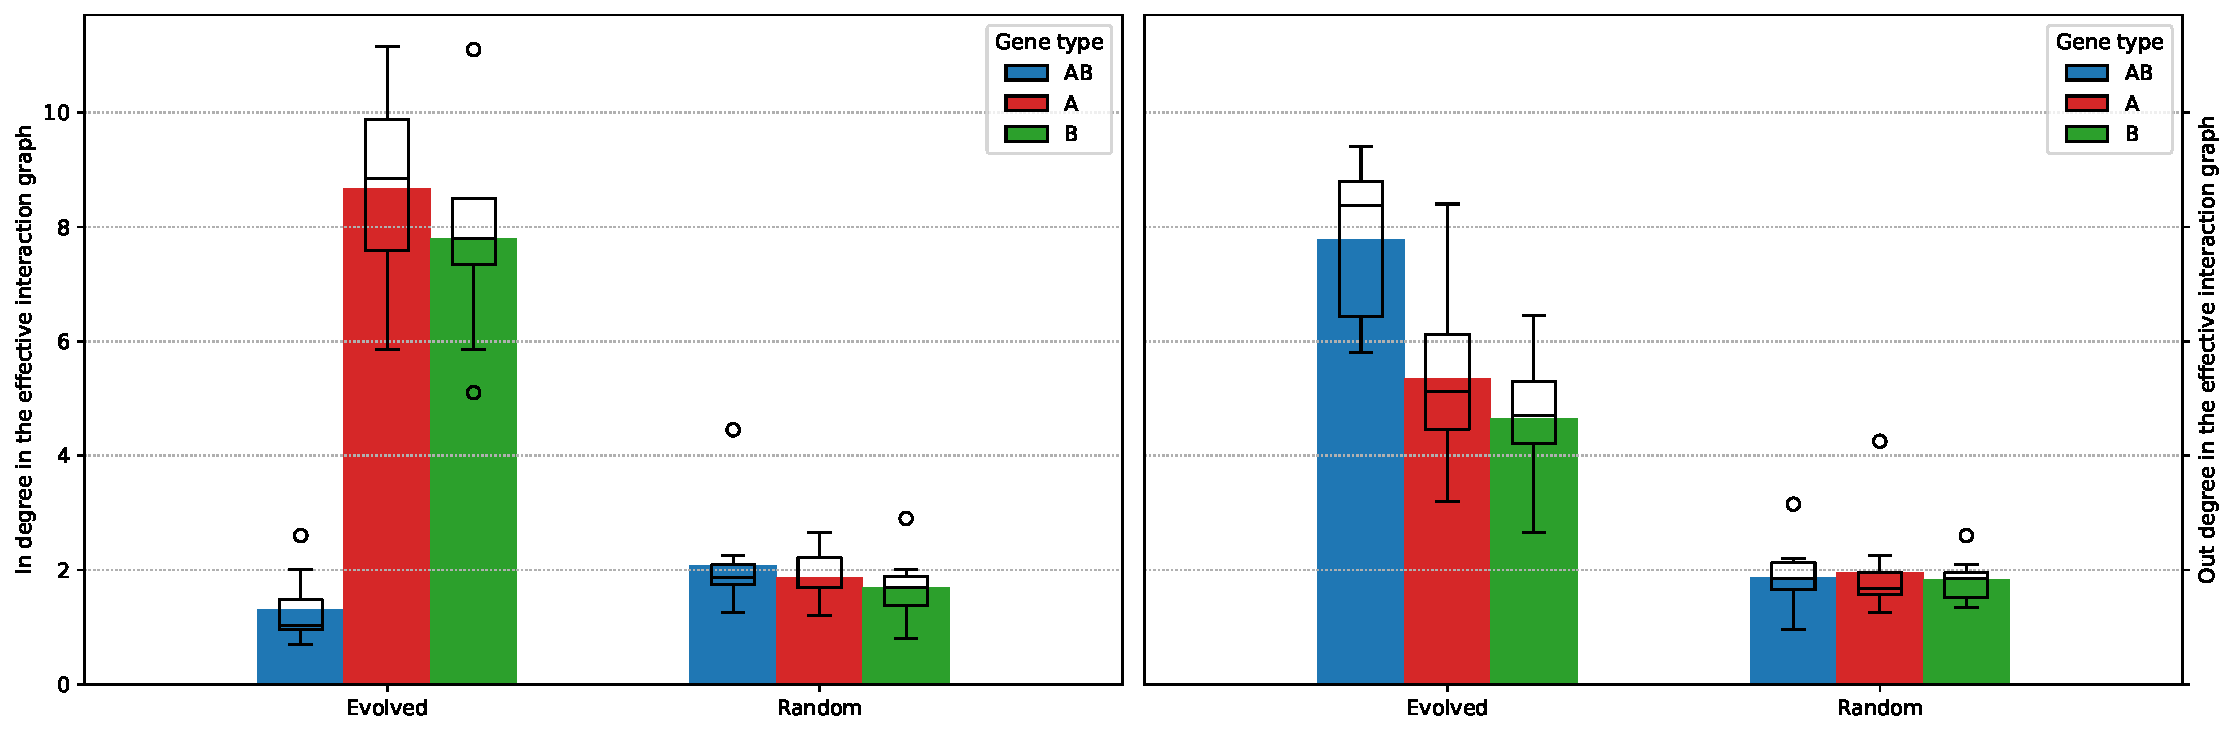
\includegraphics[width=\textwidth]{param/evolve-intergene/effective_graph_combined_degree.pdf}
\caption{Effective graph degrees at the end of evolution with intergenic distance mutations.}
\end{figure}

%\section{Mutation in Basal Supercoiling}